\documentclass{report}
%%%%%%%%%%%%%%%%%%%%%%%%%%%%%%%%%
% PACKAGE IMPORTS
%%%%%%%%%%%%%%%%%%%%%%%%%%%%%%%%%


\usepackage[tmargin=2cm,rmargin=1.5in,lmargin=1.5in,margin=0.85in,bmargin=2cm,footskip=.2in]{geometry}
\usepackage{bookmark}
\usepackage{amsmath,amsfonts,amsthm,amssymb,mathtools}
\usepackage[varbb]{newpxmath}
\usepackage{chemfig}
\usepackage{xfrac}
\usepackage{mhchem}
\usepackage[italian]{babel}
\usepackage{wrapfig}
\usepackage[makeroom]{cancel}
\usepackage{mathtools}
\usepackage{listing}
\usepackage{enumitem}
\usepackage{hyperref,theoremref}
\hypersetup{
	pdftitle={Pendolo quadrifilare e multithreading},
	colorlinks=true, linkcolor=doc!90,
	bookmarksnumbered=true,
	bookmarksopen=true
}
\usepackage[most,many,breakable]{tcolorbox}
\usepackage{xcolor}
\usepackage{varwidth}
\usepackage{varwidth}
\usepackage{etoolbox}
%\usepackage{authblk}
\usepackage{nameref}
\usepackage{multicol,array}
\usepackage{tikz-cd}
\usepackage[ruled,vlined,linesnumbered]{algorithm2e}
\usepackage{comment} % enables the use of multi-line comments (\ifx \fi) 
\usepackage{import}
\usepackage{xifthen}
\usepackage{pdfpages}
\usepackage{transparent}

%\newcommand\mycommfont[1]{\footnotesize\ttfamily\textcolor{blue}{#1}}
%\SetCommentSty{mycommfont}
%\newcommand{\incfig}[1]{%
%    \def\svgwidth{\columnwidth}
%    \import{./figures/}{#1.pdf_tex}
%}
\usepackage{pgfplots}
\usepackage{tikzsymbols}
\usepackage{float}
\renewcommand\qedsymbol{$\Laughey$}
\usepackage{hyperref}
\usepackage{siunitx}
\usepackage{imakeidx}
%\usepackage{import}
%\usepackage{xifthen}
%\usepackage{pdfpages}
%\usepackage{transparent}


%%%%%%%%%%%%%%%%%%%%%%%%%%%%%%
% SELF MADE COLORS
%%%%%%%%%%%%%%%%%%%%%%%%%%%%%%


\definecolor{doc}{RGB}{0,0,0}
\definecolor{myg}{RGB}{56, 140, 70}
\definecolor{myb}{RGB}{45, 111, 177}
\definecolor{myr}{RGB}{199, 68, 64}
\definecolor{mytheorembg}{HTML}{F2F2F9}
\definecolor{mytheoremfr}{HTML}{00007B}
\definecolor{mylenmabg}{HTML}{FFFAF8}
\definecolor{mylenmafr}{HTML}{983b0f}
\definecolor{mypropbg}{HTML}{f2fbfc}
\definecolor{mypropfr}{HTML}{191971}
\definecolor{myexamplebg}{HTML}{F2FBF8}
\definecolor{myexamplefr}{HTML}{88D6D1}
\definecolor{myexampleti}{HTML}{2A7F7F}
\definecolor{mydefinitbg}{HTML}{E5E5FF}
\definecolor{mydefinitfr}{HTML}{3F3FA3}
\definecolor{notesgreen}{RGB}{0,162,0}
\definecolor{myp}{RGB}{197, 92, 212}
\definecolor{mygr}{HTML}{2C3338}
\definecolor{myred}{RGB}{127,0,0}
\definecolor{myyellow}{RGB}{169,121,69}
\definecolor{myexercisebg}{HTML}{F2FBF8}
\definecolor{myexercisefg}{HTML}{88D6D1}

%%%%%%%%%%%%%%%%%%%%%%%%%%%%
% TCOLORBOX SETUPS
%%%%%%%%%%%%%%%%%%%%%%%%%%%%

\setlength{\parindent}{1cm}
%================================
% THEOREM BOX
%================================

\tcbuselibrary{theorems,skins,hooks}
\newtcbtheorem[number within=section]{Theorem}{Teorema}
{%
	enhanced,
	breakable,
	colback = mytheorembg,
	frame hidden,
	boxrule = 0sp,
	borderline west = {2pt}{0pt}{mytheoremfr},
	sharp corners,
	detach title,
	before upper = \tcbtitle\par\smallskip,
	coltitle = mytheoremfr,
	fonttitle = \bfseries\sffamily,
	description font = \mdseries,
	separator sign none,
	segmentation style={solid, mytheoremfr},
}
{th}

\tcbuselibrary{theorems,skins,hooks}
\newtcbtheorem[number within=chapter]{theorem}{Teorema}
{%
	enhanced,
	breakable,
	colback = mytheorembg,
	frame hidden,
	boxrule = 0sp,
	borderline west = {2pt}{0pt}{mytheoremfr},
	sharp corners,
	detach title,
	before upper = \tcbtitle\par\smallskip,
	coltitle = mytheoremfr,
	fonttitle = \bfseries\sffamily,
	description font = \mdseries,
	separator sign none,
	segmentation style={solid, mytheoremfr},
}
{th}


\tcbuselibrary{theorems,skins,hooks}
\newtcolorbox{Theoremcon}
{%
	enhanced
	,breakable
	,colback = mytheorembg
	,frame hidden
	,boxrule = 0sp
	,borderline west = {2pt}{0pt}{mytheoremfr}
	,sharp corners
	,description font = \mdseries
	,separator sign none
}

%================================
% Corollery
%================================
\tcbuselibrary{theorems,skins,hooks}
\newtcbtheorem[number within=section]{Corollary}{Corollario}
{%
	enhanced
	,breakable
	,colback = myp!10
	,frame hidden
	,boxrule = 0sp
	,borderline west = {2pt}{0pt}{myp!85!black}
	,sharp corners
	,detach title
	,before upper = \tcbtitle\par\smallskip
	,coltitle = myp!85!black
	,fonttitle = \bfseries\sffamily
	,description font = \mdseries
	,separator sign none
	,segmentation style={solid, myp!85!black}
}
{th}
\tcbuselibrary{theorems,skins,hooks}
\newtcbtheorem[number within=chapter]{corollary}{Corollario}
{%
	enhanced
	,breakable
	,colback = myp!10
	,frame hidden
	,boxrule = 0sp
	,borderline west = {2pt}{0pt}{myp!85!black}
	,sharp corners
	,detach title
	,before upper = \tcbtitle\par\smallskip
	,coltitle = myp!85!black
	,fonttitle = \bfseries\sffamily
	,description font = \mdseries
	,separator sign none
	,segmentation style={solid, myp!85!black}
}
{th}


%================================
% LENMA
%================================

\tcbuselibrary{theorems,skins,hooks}
\newtcbtheorem[number within=section]{lemna}{Lemna}
{%
	enhanced,
	breakable,
	colback = mylenmabg,
	frame hidden,
	boxrule = 0sp,
	borderline west = {2pt}{0pt}{mylenmafr},
	sharp corners,
	detach title,
	before upper = \tcbtitle\par\smallskip,
	coltitle = mylenmafr,
	fonttitle = \bfseries\sffamily,
	description font = \mdseries,
	separator sign none,
	segmentation style={solid, mylenmafr},
}
{th}

\tcbuselibrary{theorems,skins,hooks}
\newtcbtheorem[number within=chapter]{mlemma}{Lemma}
{%
	enhanced,
	breakable,
	colback = mylenmabg,
	frame hidden,
	boxrule = 0sp,
	borderline west = {2pt}{0pt}{mylenmafr},
	sharp corners,
	detach title,
	before upper = \tcbtitle\par\smallskip,
	coltitle = mylenmafr,
	fonttitle = \bfseries\sffamily,
	description font = \mdseries,
	separator sign none,
	segmentation style={solid, mylenmafr},
}
{th}


%================================
% PROPOSITION
%================================

\tcbuselibrary{theorems,skins,hooks}
\newtcbtheorem[number within=section]{Prop}{Proposizione}
{%
	enhanced,
	breakable,
	colback = mypropbg,
	frame hidden,
	boxrule = 0sp,
	borderline west = {2pt}{0pt}{mypropfr},
	sharp corners,
	detach title,
	before upper = \tcbtitle\par\smallskip,
	coltitle = mypropfr,
	fonttitle = \bfseries\sffamily,
	description font = \mdseries,
	separator sign none,
	segmentation style={solid, mypropfr},
}
{th}

\tcbuselibrary{theorems,skins,hooks}
\newtcbtheorem[number within=chapter]{prop}{Proposizione}
{%
	enhanced,
	breakable,
	colback = mypropbg,
	frame hidden,
	boxrule = 0sp,
	borderline west = {2pt}{0pt}{mypropfr},
	sharp corners,
	detach title,
	before upper = \tcbtitle\par\smallskip,
	coltitle = mypropfr,
	fonttitle = \bfseries\sffamily,
	description font = \mdseries,
	separator sign none,
	segmentation style={solid, mypropfr},
}
{th}


%================================
% CLAIM
%================================

\tcbuselibrary{theorems,skins,hooks}
\newtcbtheorem[number within=section]{claim}{Claim}
{%
	enhanced
	,breakable
	,colback = myg!10
	,frame hidden
	,boxrule = 0sp
	,borderline west = {2pt}{0pt}{myg}
	,sharp corners
	,detach title
	,before upper = \tcbtitle\par\smallskip
	,coltitle = myg!85!black
	,fonttitle = \bfseries\sffamily
	,description font = \mdseries
	,separator sign none
	,segmentation style={solid, myg!85!black}
}
{th}



%================================
% Exercise
%================================

\tcbuselibrary{theorems,skins,hooks}
\newtcbtheorem[number within=section]{Exercise}{Esercizio}
{%
	enhanced,
	breakable,
	colback = myexercisebg,
	frame hidden,
        oversize,
	boxrule = 0sp,
	borderline west = {2pt}{0pt}{myexercisefg},
	sharp corners,
	detach title,
	before upper = \tcbtitle\par\smallskip,
	coltitle = myexercisefg,
	fonttitle = \bfseries\sffamily,
	description font = \mdseries,
	separator sign none,
	segmentation style={solid, myexercisefg},
}
{th}

\tcbuselibrary{theorems,skins,hooks}
\newtcbtheorem[number within=chapter]{exercise}{Esercizio}
{%
	enhanced,
	breakable,
	colback = myexercisebg,
	frame hidden,
        oversize,
	boxrule = 0sp,
	borderline west = {2pt}{0pt}{myexercisefg},
	sharp corners,
	detach title,
	before upper = \tcbtitle\par\smallskip,
	coltitle = myexercisefg,
	fonttitle = \bfseries\sffamily,
	description font = \mdseries,
	separator sign none,
	segmentation style={solid, myexercisefg},
}
{th}
%================================
% EXAMPLE BOX
%================================

\newtcbtheorem[number within=section]{Example}{Esempio}
{%
	colback = myexamplebg
	,breakable
	,colframe = myexamplefr
	,coltitle = myexampleti
	,boxrule = 1pt
	,sharp corners
	,detach title
	,before upper=\tcbtitle\par\smallskip
	,fonttitle = \bfseries
	,description font = \mdseries
	,separator sign none
	,description delimiters parenthesis
}
{ex}

\newtcbtheorem[number within=chapter]{example}{Esempio}
{%
	colback = myexamplebg
	,breakable
	,colframe = myexamplefr
	,coltitle = myexampleti
	,boxrule = 1pt
	,sharp corners
	,detach title
	,before upper=\tcbtitle\par\smallskip
	,fonttitle = \bfseries
	,description font = \mdseries
	,separator sign none
	,description delimiters parenthesis
}
{ex}

%================================
% DEFINITION BOX
%================================

\newtcbtheorem[number within=section]{Definition}{Definizione}{enhanced,
	before skip=2mm,after skip=2mm, colback=red!5,colframe=red!80!black,boxrule=0.5mm,
	attach boxed title to top left={xshift=1cm,yshift*=1mm-\tcboxedtitleheight}, varwidth boxed title*=-3cm,
	boxed title style={frame code={
					\path[fill=tcbcolback]
					([yshift=-1mm,xshift=-1mm]frame.north west)
					arc[start angle=0,end angle=180,radius=1mm]
					([yshift=-1mm,xshift=1mm]frame.north east)
					arc[start angle=180,end angle=0,radius=1mm];
					\path[left color=tcbcolback!60!black,right color=tcbcolback!60!black,
						middle color=tcbcolback!80!black]
					([xshift=-2mm]frame.north west) -- ([xshift=2mm]frame.north east)
					[rounded corners=1mm]-- ([xshift=1mm,yshift=-1mm]frame.north east)
					-- (frame.south east) -- (frame.south west)
					-- ([xshift=-1mm,yshift=-1mm]frame.north west)
					[sharp corners]-- cycle;
				},interior engine=empty,
		},
	fonttitle=\bfseries,
	title={#2},#1}{def}
\newtcbtheorem[number within=chapter]{definition}{Definizione}{enhanced,
	before skip=2mm,after skip=2mm, colback=red!5,colframe=red!80!black,boxrule=0.5mm,
	attach boxed title to top left={xshift=1cm,yshift*=1mm-\tcboxedtitleheight}, varwidth boxed title*=-3cm,
	boxed title style={frame code={
					\path[fill=tcbcolback]
					([yshift=-1mm,xshift=-1mm]frame.north west)
					arc[start angle=0,end angle=180,radius=1mm]
					([yshift=-1mm,xshift=1mm]frame.north east)
					arc[start angle=180,end angle=0,radius=1mm];
					\path[left color=tcbcolback!60!black,right color=tcbcolback!60!black,
						middle color=tcbcolback!80!black]
					([xshift=-2mm]frame.north west) -- ([xshift=2mm]frame.north east)
					[rounded corners=1mm]-- ([xshift=1mm,yshift=-1mm]frame.north east)
					-- (frame.south east) -- (frame.south west)
					-- ([xshift=-1mm,yshift=-1mm]frame.north west)
					[sharp corners]-- cycle;
				},interior engine=empty,
		},
	fonttitle=\bfseries,
	title={#2},#1}{def}



%================================
% Question BOX
%================================

\makeatletter
\newtcbtheorem{question}{Domanda}{enhanced,
	breakable,
	colback=white,
	colframe=myb!80!black,
	attach boxed title to top left={yshift*=-\tcboxedtitleheight},
	fonttitle=\bfseries,
	title={#2},
	boxed title size=title,
	boxed title style={%
			sharp corners,
			rounded corners=northwest,
			colback=tcbcolframe,
			boxrule=0pt,
		},
	underlay boxed title={%
			\path[fill=tcbcolframe] (title.south west)--(title.south east)
			to[out=0, in=180] ([xshift=5mm]title.east)--
			(title.center-|frame.east)
			[rounded corners=\kvtcb@arc] |-
			(frame.north) -| cycle;
		},
	#1
}{def}
\makeatother

%================================
% SOLUTION BOX
%================================

\makeatletter
\newtcolorbox{solution}{enhanced,
	breakable,
	colback=white,
	colframe=myg!80!black,
	attach boxed title to top left={yshift*=-\tcboxedtitleheight},
	title=Soluzione,
	boxed title size=title,
	boxed title style={%
			sharp corners,
			rounded corners=northwest,
			colback=tcbcolframe,
			boxrule=0pt,
		},
	underlay boxed title={%
			\path[fill=tcbcolframe] (title.south west)--(title.south east)
			to[out=0, in=180] ([xshift=5mm]title.east)--
			(title.center-|frame.east)
			[rounded corners=\kvtcb@arc] |-
			(frame.north) -| cycle;
		},
}
\makeatother

%================================
% Question BOX
%================================

\makeatletter
\newtcbtheorem{qstion}{Risposta}{enhanced,
	breakable,
	colback=white,
	colframe=mygr,
	attach boxed title to top left={yshift*=-\tcboxedtitleheight},
	fonttitle=\bfseries,
	title={#2},
	boxed title size=title,
	boxed title style={%
			sharp corners,
			rounded corners=northwest,
			colback=tcbcolframe,
			boxrule=0pt,
		},
	underlay boxed title={%
			\path[fill=tcbcolframe] (title.south west)--(title.south east)
			to[out=0, in=180] ([xshift=5mm]title.east)--
			(title.center-|frame.east)
			[rounded corners=\kvtcb@arc] |-
			(frame.north) -| cycle;
		},
	#1
}{def}
\makeatother

\newtcbtheorem[number within=chapter]{wconc}{Wrong Concept}{
	breakable,
	enhanced,
	colback=white,
	colframe=myr,
	arc=0pt,
	outer arc=0pt,
	fonttitle=\bfseries\sffamily\large,
	colbacktitle=myr,
	attach boxed title to top left={},
	boxed title style={
			enhanced,
			skin=enhancedfirst jigsaw,
			arc=3pt,
			bottom=0pt,
			interior style={fill=myr}
		},
	#1
}{def}



%================================
% NOTE BOX
%================================

\usetikzlibrary{arrows,calc,shadows.blur}
\tcbuselibrary{skins}
\newtcolorbox{note}[1][]{%
	enhanced jigsaw,
	colback=gray!20!white,%
	colframe=gray!80!black,
	size=small,
	boxrule=1pt,
	title=\textbf{Osservazione:-},
	halign title=flush center,
	coltitle=black,
	breakable,
	drop shadow=black!50!white,
	attach boxed title to top left={xshift=1cm,yshift=-\tcboxedtitleheight/2,yshifttext=-\tcboxedtitleheight/2},
	minipage boxed title=3.5cm,
	boxed title style={%
			colback=white,
			size=fbox,
			boxrule=1pt,
			boxsep=2pt,
			underlay={%
					\coordinate (dotA) at ($(interior.west) + (-0.5pt,0)$);
					\coordinate (dotB) at ($(interior.east) + (0.5pt,0)$);
					\begin{scope}
						\clip (interior.north west) rectangle ([xshift=3ex]interior.east);
						\filldraw [white, blur shadow={shadow opacity=60, shadow yshift=-.75ex}, rounded corners=2pt] (interior.north west) rectangle (interior.south east);
					\end{scope}
					\begin{scope}[gray!80!black]
						\fill (dotA) circle (2pt);
						\fill (dotB) circle (2pt);
					\end{scope}
				},
		},
	#1,
}

%%%%%%%%%%%%%%%%%%%%%%%%%%%%%%
% SELF MADE COMMANDS
%%%%%%%%%%%%%%%%%%%%%%%%%%%%%%


\newcommand{\thm}[2]{\begin{theorem}{#1}{}#2\end{theorem}}
\newcommand{\cor}[2]{\begin{corollary}{#1}{}#2\end{corollary}}
\newcommand{\lemma}[2]{\begin{lemna}{#1}{}#2\end{lemna}}
\newcommand{\mprop}[2]{\begin{prop}{#1}{}#2\end{prop}}
\newcommand{\clm}[3]{\begin{claim}{#1}{#2}#3\end{claim}}
\newcommand{\wc}[2]{\begin{wconc}{#1}{}\setlength{\parindent}{1cm}#2\end{wconc}}
\newcommand{\thmcon}[1]{\begin{Theoremcon}{#1}\end{Theoremcon}}
\newcommand{\ex}[2]{\begin{example}{#1}{}#2\end{example}}
\newcommand{\exc}[2]{\begin{Exercise}{#1}{}#2\end{Exercise}}
%\newcommand{\dfn}[2]{\begin{Definition}[colbacktitle=red!75!black]{#1}{}#2\end{Definition}}
\newcommand{\dfn}[2]{\begin{definition}[colbacktitle=red!75!black]{#1}{}#2\end{definition}}
\newcommand{\qs}[2]{\begin{question}{#1}{}#2\end{question}}
\newcommand{\pf}[2]{\begin{myproof}[#1]#2\end{myproof}}
\newcommand{\nt}[1]{\begin{note}#1\end{note}}

\newcommand*\circled[1]{\tikz[baseline=(char.base)]{
		\node[shape=circle,draw,inner sep=1pt] (char) {#1};}}
\newcommand\getcurrentref[1]{%
	\ifnumequal{\value{#1}}{0}
	{??}
	{\the\value{#1}}%
}
\newcommand{\getCurrentSectionNumber}{\getcurrentref{section}}
\newenvironment{myproof}[1][\proofname]{%
	\proof[\bfseries #1: ]%
}{\endproof}

\newcommand{\mclm}[2]{\begin{myclaim}[#1]#2\end{myclaim}}
\newenvironment{myclaim}[1][\claimname]{\proof[\bfseries #1: ]}{}

\newcounter{mylabelcounter}

\makeatletter
\newcommand{\setword}[2]{%
	\phantomsection
	#1\def\@currentlabel{\unexpanded{#1}}\label{#2}%
}
\makeatother




\tikzset{
	symbol/.style={
			draw=none,
			every to/.append style={
					edge node={node [sloped, allow upside down, auto=false]{$#1$}}}
		}
}


% deliminators
\DeclarePairedDelimiter{\abs}{\lvert}{\rvert}
\DeclarePairedDelimiter{\norm}{\lVert}{\rVert}

\DeclarePairedDelimiter{\ceil}{\lceil}{\rceil}
\DeclarePairedDelimiter{\floor}{\lfloor}{\rfloor}
\DeclarePairedDelimiter{\round}{\lfloor}{\rceil}

\newsavebox\diffdbox
\newcommand{\slantedromand}{{\mathpalette\makesl{d}}}
\newcommand{\makesl}[2]{%
\begingroup
\sbox{\diffdbox}{$\mathsurround=0pt#1\mathrm{#2}$}%
\pdfsave
\pdfsetmatrix{1 0 0.2 1}%
\rlap{\usebox{\diffdbox}}%
\pdfrestore
\hskip\wd\diffdbox
\endgroup
}
\newcommand{\dd}[1][]{\ensuremath{\mathop{}\!\ifstrempty{#1}{%
\slantedromand\@ifnextchar^{\hspace{0.2ex}}{\hspace{0.1ex}}}%
{\slantedromand\hspace{0.2ex}^{#1}}}}
\ProvideDocumentCommand\dv{o m g}{%
  \ensuremath{%
    \IfValueTF{#3}{%
      \IfNoValueTF{#1}{%
        \frac{\dd #2}{\dd #3}%
      }{%
        \frac{\dd^{#1} #2}{\dd #3^{#1}}%
      }%
    }{%
      \IfNoValueTF{#1}{%
        \frac{\dd}{\dd #2}%
      }{%
        \frac{\dd^{#1}}{\dd #2^{#1}}%
      }%
    }%
  }%
}
\providecommand*{\pdv}[3][]{\frac{\partial^{#1}#2}{\partial#3^{#1}}}
%  - others
\DeclareMathOperator{\Lap}{\mathcal{L}}
\DeclareMathOperator{\Var}{Var} % varience
\DeclareMathOperator{\Cov}{Cov} % covarience
\DeclareMathOperator{\E}{E} % expected

% Since the amsthm package isn't loaded

% I prefer the slanted \leq
\let\oldleq\leq % save them in case they're every wanted
\let\oldgeq\geq
\renewcommand{\leq}{\leqslant}
\renewcommand{\geq}{\geqslant}

% % redefine matrix env to allow for alignment, use r as default
% \renewcommand*\env@matrix[1][r]{\hskip -\arraycolsep
%     \let\@ifnextchar\new@ifnextchar
%     \array{*\c@MaxMatrixCols #1}}


%\usepackage{framed}
%\usepackage{titletoc}
%\usepackage{etoolbox}
%\usepackage{lmodern}


%\patchcmd{\tableofcontents}{\contentsname}{\sffamily\contentsname}{}{}

%\renewenvironment{leftbar}
%{\def\FrameCommand{\hspace{6em}%
%		{\color{myyellow}\vrule width 2pt depth 6pt}\hspace{1em}}%
%	\MakeFramed{\parshape 1 0cm \dimexpr\textwidth-6em\relax\FrameRestore}\vskip2pt%
%}
%{\endMakeFramed}

%\titlecontents{chapter}
%[0em]{\vspace*{2\baselineskip}}
%{\parbox{4.5em}{%
%		\hfill\Huge\sffamily\bfseries\color{myred}\thecontentspage}%
%	\vspace*{-2.3\baselineskip}\leftbar\textsc{\small\chaptername~\thecontentslabel}\\\sffamily}
%{}{\endleftbar}
%\titlecontents{section}
%[8.4em]
%{\sffamily\contentslabel{3em}}{}{}
%{\hspace{0.5em}\nobreak\itshape\color{myred}\contentspage}
%\titlecontents{subsection}
%[8.4em]
%{\sffamily\contentslabel{3em}}{}{}  
%{\hspace{0.5em}\nobreak\itshape\color{myred}\contentspage}



%%%%%%%%%%%%%%%%%%%%%%%%%%%%%%%%%%%%%%%%%%%
% TABLE OF CONTENTS
%%%%%%%%%%%%%%%%%%%%%%%%%%%%%%%%%%%%%%%%%%%

\usepackage{tikz}
\definecolor{doc}{RGB}{0,0,0}
\definecolor{pink_flyod}{RGB}{252, 49, 153}
\usepackage{titletoc}
\contentsmargin{0cm}
\titlecontents{chapter}[3.7pc]
{\addvspace{30pt}%
	\begin{tikzpicture}[remember picture, overlay]%
		\draw[fill=doc!60,draw=doc!60] (-7,-.1) rectangle (-0.9,.5);%
		\pgftext[left,x=-3.5cm,y=0.2cm]{\color{white}\Large\sc\bfseries Capitolo\ \thecontentslabel};%
	\end{tikzpicture}\color{doc!60}\large\sc\bfseries}%
{}
{}
{\;\titlerule\;\large\sc\bfseries Pagina \thecontentspage
	\begin{tikzpicture}[remember picture, overlay]
		\draw[fill=doc!60,draw=doc!60] (2pt,0) rectangle (4,0.1pt);
	\end{tikzpicture}}%
\titlecontents{section}[3.7pc]
{\addvspace{2pt}}
{\contentslabel[\thecontentslabel]{2pc}}
{}
{\hfill\small \thecontentspage}
[]
\titlecontents*{subsection}[3.7pc]
{\addvspace{-1pt}\small}
{}
{}
{\ --- \small\thecontentspage}
[ \textbullet\ ][]

\makeatletter
\renewcommand{\tableofcontents}{%
	\chapter*{%
	  \vspace*{-20\p@}%
	  \begin{tikzpicture}[remember picture, overlay]%
		  \pgftext[right,x=15cm,y=0.2cm]{\color{doc!60}\Huge\sc\bfseries \contentsname};%
		  \draw[fill=doc!60,draw=doc!60] (13,-.75) rectangle (20,1);%
		  \clip (13,-.75) rectangle (20,1);
		  \pgftext[right,x=15cm,y=0.2cm]{\color{white}\Huge\sc\bfseries \contentsname};%
	  \end{tikzpicture}}%
	\@starttoc{toc}}
\makeatother

%%%%%%%%%%%%%%%%%%%%%%%%
% QUOTE
%%%%%%%%%%%%%%%%%%%%%%%%
\newtcolorbox{zitat}[1][]{%
    after={\par\smallskip\noindent},
    colback=white,
    frame hidden,
    grow to right by=-10mm,
    grow to left by=-10mm, 
    boxrule=0pt,
    boxsep=0pt,
    breakable,
    enhanced jigsaw,
    borderline west={0.5pt}{0pt}{black},
    colbacktitle={white},
    coltitle={black},
    fonttitle={\large\bfseries},
}
\newcommand{\qte}[1]{\begin{zitat} #1 \end{zitat}}

%%%%%%%%%%%%%%%%%%%%%%%%%
% LSTLISTINGS COLORS
%%%%%%%%%%%%%%%%%%%%%%%%%
\definecolor{codegreen}{rgb}{0,0.6,0}
\definecolor{codegray}{rgb}{0.5,0.5,0.5}
\definecolor{codepurple}{rgb}{0.58,0,0.82}
\definecolor{backcolour}{rgb}{0.95,0.95,0.92}

\lstdefinestyle{code}{
    backgroundcolor=\color{backcolour},   
    commentstyle=\color{codegreen},
    keywordstyle=\color{magenta},
    numberstyle=\tiny\color{codegray},
    stringstyle=\color{codepurple},
    basicstyle=\ttfamily\footnotesize,
    breakatwhitespace=false,         
    breaklines=true,                 
    captionpos=b,                    
    keepspaces=true,                                     
    showspaces=false,                
    showstringspaces=false,
    showtabs=false,
    numbers=left,
    tabsize=2
}

\lstset{style=code}
%From M275 "Topology" at SJSU
\newcommand{\id}{\mathrm{id}}
\newcommand{\taking}[1]{\xrightarrow{#1}}
\newcommand{\inv}{^{-1}}

%From M170 "Introduction to Graph Theory" at SJSU
\DeclareMathOperator{\diam}{diam}
\DeclareMathOperator{\ord}{ord}
\newcommand{\defeq}{\overset{\mathrm{def}}{=}}

%From the USAMO .tex files
\newcommand{\ts}{\textsuperscript}
\newcommand{\dg}{^\circ}
\newcommand{\ii}{\item}

% % From Math 55 and Math 145 at Harvard
% \newenvironment{subproof}[1][Proof]{%
% \begin{proof}[#1] \renewcommand{\qedsymbol}{$\blacksquare$}}%
% {\end{proof}}

\newcommand{\liff}{\leftrightarrow}
\newcommand{\lthen}{\rightarrow}
\newcommand{\opname}{\operatorname}
\newcommand{\surjto}{\twoheadrightarrow}
\newcommand{\injto}{\hookrightarrow}
\newcommand{\On}{\mathrm{On}} % ordinals
\DeclareMathOperator{\img}{im} % Image
\DeclareMathOperator{\Img}{Im} % Image
\DeclareMathOperator{\coker}{coker} % Cokernel
\DeclareMathOperator{\Coker}{Coker} % Cokernel
\DeclareMathOperator{\Ker}{Ker} % Kernel
\DeclareMathOperator{\rank}{rank}
\DeclareMathOperator{\Spec}{Spec} % spectrum
\DeclareMathOperator{\Tr}{Tr} % trace
\DeclareMathOperator{\pr}{pr} % projection
\DeclareMathOperator{\ext}{ext} % extension
\DeclareMathOperator{\pred}{pred} % predecessor
\DeclareMathOperator{\dom}{dom} % domain
\DeclareMathOperator{\ran}{ran} % range
\DeclareMathOperator{\Hom}{Hom} % homomorphism
\DeclareMathOperator{\Mor}{Mor} % morphisms
\DeclareMathOperator{\End}{End} % endomorphism

\newcommand{\eps}{\epsilon}
\newcommand{\veps}{\varepsilon}
\newcommand{\ol}{\overline}
\newcommand{\ul}{\underline}
\newcommand{\wt}{\widetilde}
\newcommand{\wh}{\widehat}
\newcommand{\vocab}[1]{\textbf{\color{blue} #1}}
\providecommand{\half}{\frac{1}{2}}
\newcommand{\dang}{\measuredangle} %% Directed angle
\newcommand{\ray}[1]{\overrightarrow{#1}}
\newcommand{\seg}[1]{\overline{#1}}
\newcommand{\arc}[1]{\wideparen{#1}}
\DeclareMathOperator{\cis}{cis}
\DeclareMathOperator*{\lcm}{lcm}
\DeclareMathOperator*{\argmin}{arg min}
\DeclareMathOperator*{\argmax}{arg max}
\newcommand{\cycsum}{\sum_{\mathrm{cyc}}}
\newcommand{\symsum}{\sum_{\mathrm{sym}}}
\newcommand{\cycprod}{\prod_{\mathrm{cyc}}}
\newcommand{\symprod}{\prod_{\mathrm{sym}}}
\newcommand{\Qed}{\begin{flushright}\qed\end{flushright}}
\newcommand{\parinn}{\setlength{\parindent}{1cm}}
\newcommand{\parinf}{\setlength{\parindent}{0cm}}
% \newcommand{\norm}{\|\cdot\|}
\newcommand{\inorm}{\norm_{\infty}}
\newcommand{\opensets}{\{V_{\alpha}\}_{\alpha\in I}}
\newcommand{\oset}{V_{\alpha}}
\newcommand{\opset}[1]{V_{\alpha_{#1}}}
\newcommand{\lub}{\text{lub}}
\newcommand{\del}[2]{\frac{\partial #1}{\partial #2}}
\newcommand{\Del}[3]{\frac{\partial^{#1} #2}{\partial^{#1} #3}}
\newcommand{\deld}[2]{\dfrac{\partial #1}{\partial #2}}
\newcommand{\Deld}[3]{\dfrac{\partial^{#1} #2}{\partial^{#1} #3}}
\newcommand{\lm}{\lambda}
\newcommand{\uin}{\mathbin{\rotatebox[origin=c]{90}{$\in$}}}
\newcommand{\usubset}{\mathbin{\rotatebox[origin=c]{90}{$\subset$}}}
\newcommand{\lt}{\left}
\newcommand{\rt}{\right}
\newcommand{\bs}[1]{\boldsymbol{#1}}
\newcommand{\exs}{\exists}
\newcommand{\st}{\strut}
\newcommand{\dps}[1]{\displaystyle{#1}}

\newcommand{\sol}{\setlength{\parindent}{0cm}\textbf{\textit{Soluzione:}}\setlength{\parindent}{1cm} }
\newcommand{\solve}[1]{\setlength{\parindent}{0cm}\textbf{\textit{Soluzione: }}\setlength{\parindent}{1cm}#1 \Qed}

% Things Lie
\newcommand{\kb}{\mathfrak b}
\newcommand{\kg}{\mathfrak g}
\newcommand{\kh}{\mathfrak h}
\newcommand{\kn}{\mathfrak n}
\newcommand{\ku}{\mathfrak u}
\newcommand{\kz}{\mathfrak z}
\DeclareMathOperator{\Ext}{Ext} % Ext functor
\DeclareMathOperator{\Tor}{Tor} % Tor functor
\newcommand{\gl}{\opname{\mathfrak{gl}}} % frak gl group
\renewcommand{\sl}{\opname{\mathfrak{sl}}} % frak sl group chktex 6

% More script letters etc.
\newcommand{\SA}{\mathcal A}
\newcommand{\SB}{\mathcal B}
\newcommand{\SC}{\mathcal C}
\newcommand{\SF}{\mathcal F}
\newcommand{\SG}{\mathcal G}
\newcommand{\SH}{\mathcal H}
\newcommand{\OO}{\mathcal O}

\newcommand{\SCA}{\mathscr A}
\newcommand{\SCB}{\mathscr B}
\newcommand{\SCC}{\mathscr C}
\newcommand{\SCD}{\mathscr D}
\newcommand{\SCE}{\mathscr E}
\newcommand{\SCF}{\mathscr F}
\newcommand{\SCG}{\mathscr G}
\newcommand{\SCH}{\mathscr H}

% Mathfrak primes
\newcommand{\km}{\mathfrak m}
\newcommand{\kp}{\mathfrak p}
\newcommand{\kq}{\mathfrak q}

% number sets
\newcommand{\RR}[1][]{\ensuremath{\ifstrempty{#1}{\mathbb{R}}{\mathbb{R}^{#1}}}}
\newcommand{\NN}[1][]{\ensuremath{\ifstrempty{#1}{\mathbb{N}}{\mathbb{N}^{#1}}}}
\newcommand{\ZZ}[1][]{\ensuremath{\ifstrempty{#1}{\mathbb{Z}}{\mathbb{Z}^{#1}}}}
\newcommand{\QQ}[1][]{\ensuremath{\ifstrempty{#1}{\mathbb{Q}}{\mathbb{Q}^{#1}}}}
\newcommand{\CC}[1][]{\ensuremath{\ifstrempty{#1}{\mathbb{C}}{\mathbb{C}^{#1}}}}
\newcommand{\PP}[1][]{\ensuremath{\ifstrempty{#1}{\mathbb{P}}{\mathbb{P}^{#1}}}}
\newcommand{\HH}[1][]{\ensuremath{\ifstrempty{#1}{\mathbb{H}}{\mathbb{H}^{#1}}}}
\newcommand{\FF}[1][]{\ensuremath{\ifstrempty{#1}{\mathbb{F}}{\mathbb{F}^{#1}}}}
% expected value
\newcommand{\EE}{\ensuremath{\mathbb{E}}}
\newcommand{\charin}{\text{ char }}
\DeclareMathOperator{\sign}{sign}
\DeclareMathOperator{\Aut}{Aut}
\DeclareMathOperator{\Inn}{Inn}
\DeclareMathOperator{\Syl}{Syl}
\DeclareMathOperator{\Gal}{Gal}
\DeclareMathOperator{\GL}{GL} % General linear group
\DeclareMathOperator{\SL}{SL} % Special linear group

%---------------------------------------
% BlackBoard Math Fonts :-
%---------------------------------------

%Captital Letters
\newcommand{\bbA}{\mathbb{A}}	\newcommand{\bbB}{\mathbb{B}}
\newcommand{\bbC}{\mathbb{C}}	\newcommand{\bbD}{\mathbb{D}}
\newcommand{\bbE}{\mathbb{E}}	\newcommand{\bbF}{\mathbb{F}}
\newcommand{\bbG}{\mathbb{G}}	\newcommand{\bbH}{\mathbb{H}}
\newcommand{\bbI}{\mathbb{I}}	\newcommand{\bbJ}{\mathbb{J}}
\newcommand{\bbK}{\mathbb{K}}	\newcommand{\bbL}{\mathbb{L}}
\newcommand{\bbM}{\mathbb{M}}	\newcommand{\bbN}{\mathbb{N}}
\newcommand{\bbO}{\mathbb{O}}	\newcommand{\bbP}{\mathbb{P}}
\newcommand{\bbQ}{\mathbb{Q}}	\newcommand{\bbR}{\mathbb{R}}
\newcommand{\bbS}{\mathbb{S}}	\newcommand{\bbT}{\mathbb{T}}
\newcommand{\bbU}{\mathbb{U}}	\newcommand{\bbV}{\mathbb{V}}
\newcommand{\bbW}{\mathbb{W}}	\newcommand{\bbX}{\mathbb{X}}
\newcommand{\bbY}{\mathbb{Y}}	\newcommand{\bbZ}{\mathbb{Z}}

%---------------------------------------
% MathCal Fonts :-
%---------------------------------------

%Captital Letters
\newcommand{\mcA}{\mathcal{A}}	\newcommand{\mcB}{\mathcal{B}}
\newcommand{\mcC}{\mathcal{C}}	\newcommand{\mcD}{\mathcal{D}}
\newcommand{\mcE}{\mathcal{E}}	\newcommand{\mcF}{\mathcal{F}}
\newcommand{\mcG}{\mathcal{G}}	\newcommand{\mcH}{\mathcal{H}}
\newcommand{\mcI}{\mathcal{I}}	\newcommand{\mcJ}{\mathcal{J}}
\newcommand{\mcK}{\mathcal{K}}	\newcommand{\mcL}{\mathcal{L}}
\newcommand{\mcM}{\mathcal{M}}	\newcommand{\mcN}{\mathcal{N}}
\newcommand{\mcO}{\mathcal{O}}	\newcommand{\mcP}{\mathcal{P}}
\newcommand{\mcQ}{\mathcal{Q}}	\newcommand{\mcR}{\mathcal{R}}
\newcommand{\mcS}{\mathcal{S}}	\newcommand{\mcT}{\mathcal{T}}
\newcommand{\mcU}{\mathcal{U}}	\newcommand{\mcV}{\mathcal{V}}
\newcommand{\mcW}{\mathcal{W}}	\newcommand{\mcX}{\mathcal{X}}
\newcommand{\mcY}{\mathcal{Y}}	\newcommand{\mcZ}{\mathcal{Z}}


%---------------------------------------
% Bold Math Fonts :-
%---------------------------------------

%Captital Letters
\newcommand{\bmA}{\boldsymbol{A}}	\newcommand{\bmB}{\boldsymbol{B}}
\newcommand{\bmC}{\boldsymbol{C}}	\newcommand{\bmD}{\boldsymbol{D}}
\newcommand{\bmE}{\boldsymbol{E}}	\newcommand{\bmF}{\boldsymbol{F}}
\newcommand{\bmG}{\boldsymbol{G}}	\newcommand{\bmH}{\boldsymbol{H}}
\newcommand{\bmI}{\boldsymbol{I}}	\newcommand{\bmJ}{\boldsymbol{J}}
\newcommand{\bmK}{\boldsymbol{K}}	\newcommand{\bmL}{\boldsymbol{L}}
\newcommand{\bmM}{\boldsymbol{M}}	\newcommand{\bmN}{\boldsymbol{N}}
\newcommand{\bmO}{\boldsymbol{O}}	\newcommand{\bmP}{\boldsymbol{P}}
\newcommand{\bmQ}{\boldsymbol{Q}}	\newcommand{\bmR}{\boldsymbol{R}}
\newcommand{\bmS}{\boldsymbol{S}}	\newcommand{\bmT}{\boldsymbol{T}}
\newcommand{\bmU}{\boldsymbol{U}}	\newcommand{\bmV}{\boldsymbol{V}}
\newcommand{\bmW}{\boldsymbol{W}}	\newcommand{\bmX}{\boldsymbol{X}}
\newcommand{\bmY}{\boldsymbol{Y}}	\newcommand{\bmZ}{\boldsymbol{Z}}
%Small Letters
\newcommand{\bma}{\boldsymbol{a}}	\newcommand{\bmb}{\boldsymbol{b}}
\newcommand{\bmc}{\boldsymbol{c}}	\newcommand{\bmd}{\boldsymbol{d}}
\newcommand{\bme}{\boldsymbol{e}}	\newcommand{\bmf}{\boldsymbol{f}}
\newcommand{\bmg}{\boldsymbol{g}}	\newcommand{\bmh}{\boldsymbol{h}}
\newcommand{\bmi}{\boldsymbol{i}}	\newcommand{\bmj}{\boldsymbol{j}}
\newcommand{\bmk}{\boldsymbol{k}}	\newcommand{\bml}{\boldsymbol{l}}
\newcommand{\bmm}{\boldsymbol{m}}	\newcommand{\bmn}{\boldsymbol{n}}
\newcommand{\bmo}{\boldsymbol{o}}	\newcommand{\bmp}{\boldsymbol{p}}
\newcommand{\bmq}{\boldsymbol{q}}	\newcommand{\bmr}{\boldsymbol{r}}
\newcommand{\bms}{\boldsymbol{s}}	\newcommand{\bmt}{\boldsymbol{t}}
\newcommand{\bmu}{\boldsymbol{u}}	\newcommand{\bmv}{\boldsymbol{v}}
\newcommand{\bmw}{\boldsymbol{w}}	\newcommand{\bmx}{\boldsymbol{x}}
\newcommand{\bmy}{\boldsymbol{y}}	\newcommand{\bmz}{\boldsymbol{z}}

%---------------------------------------
% Scr Math Fonts :-
%---------------------------------------

\newcommand{\sA}{{\mathscr{A}}}   \newcommand{\sB}{{\mathscr{B}}}
\newcommand{\sC}{{\mathscr{C}}}   \newcommand{\sD}{{\mathscr{D}}}
\newcommand{\sE}{{\mathscr{E}}}   \newcommand{\sF}{{\mathscr{F}}}
\newcommand{\sG}{{\mathscr{G}}}   \newcommand{\sH}{{\mathscr{H}}}
\newcommand{\sI}{{\mathscr{I}}}   \newcommand{\sJ}{{\mathscr{J}}}
\newcommand{\sK}{{\mathscr{K}}}   \newcommand{\sL}{{\mathscr{L}}}
\newcommand{\sM}{{\mathscr{M}}}   \newcommand{\sN}{{\mathscr{N}}}
\newcommand{\sO}{{\mathscr{O}}}   \newcommand{\sP}{{\mathscr{P}}}
\newcommand{\sQ}{{\mathscr{Q}}}   \newcommand{\sR}{{\mathscr{R}}}
\newcommand{\sS}{{\mathscr{S}}}   \newcommand{\sT}{{\mathscr{T}}}
\newcommand{\sU}{{\mathscr{U}}}   \newcommand{\sV}{{\mathscr{V}}}
\newcommand{\sW}{{\mathscr{W}}}   \newcommand{\sX}{{\mathscr{X}}}
\newcommand{\sY}{{\mathscr{Y}}}   \newcommand{\sZ}{{\mathscr{Z}}}


%---------------------------------------
% Math Fraktur Font
%---------------------------------------

%Captital Letters
\newcommand{\mfA}{\mathfrak{A}}	\newcommand{\mfB}{\mathfrak{B}}
\newcommand{\mfC}{\mathfrak{C}}	\newcommand{\mfD}{\mathfrak{D}}
\newcommand{\mfE}{\mathfrak{E}}	\newcommand{\mfF}{\mathfrak{F}}
\newcommand{\mfG}{\mathfrak{G}}	\newcommand{\mfH}{\mathfrak{H}}
\newcommand{\mfI}{\mathfrak{I}}	\newcommand{\mfJ}{\mathfrak{J}}
\newcommand{\mfK}{\mathfrak{K}}	\newcommand{\mfL}{\mathfrak{L}}
\newcommand{\mfM}{\mathfrak{M}}	\newcommand{\mfN}{\mathfrak{N}}
\newcommand{\mfO}{\mathfrak{O}}	\newcommand{\mfP}{\mathfrak{P}}
\newcommand{\mfQ}{\mathfrak{Q}}	\newcommand{\mfR}{\mathfrak{R}}
\newcommand{\mfS}{\mathfrak{S}}	\newcommand{\mfT}{\mathfrak{T}}
\newcommand{\mfU}{\mathfrak{U}}	\newcommand{\mfV}{\mathfrak{V}}
\newcommand{\mfW}{\mathfrak{W}}	\newcommand{\mfX}{\mathfrak{X}}
\newcommand{\mfY}{\mathfrak{Y}}	\newcommand{\mfZ}{\mathfrak{Z}}
%Small Letters
\newcommand{\mfa}{\mathfrak{a}}	\newcommand{\mfb}{\mathfrak{b}}
\newcommand{\mfc}{\mathfrak{c}}	\newcommand{\mfd}{\mathfrak{d}}
\newcommand{\mfe}{\mathfrak{e}}	\newcommand{\mff}{\mathfrak{f}}
\newcommand{\mfg}{\mathfrak{g}}	\newcommand{\mfh}{\mathfrak{h}}
\newcommand{\mfi}{\mathfrak{i}}	\newcommand{\mfj}{\mathfrak{j}}
\newcommand{\mfk}{\mathfrak{k}}	\newcommand{\mfl}{\mathfrak{l}}
\newcommand{\mfm}{\mathfrak{m}}	\newcommand{\mfn}{\mathfrak{n}}
\newcommand{\mfo}{\mathfrak{o}}	\newcommand{\mfp}{\mathfrak{p}}
\newcommand{\mfq}{\mathfrak{q}}	\newcommand{\mfr}{\mathfrak{r}}
\newcommand{\mfs}{\mathfrak{s}}	\newcommand{\mft}{\mathfrak{t}}
\newcommand{\mfu}{\mathfrak{u}}	\newcommand{\mfv}{\mathfrak{v}}
\newcommand{\mfw}{\mathfrak{w}}	\newcommand{\mfx}{\mathfrak{x}}
\newcommand{\mfy}{\mathfrak{y}}	\newcommand{\mfz}{\mathfrak{z}}

\makeindex

\title{Pendolo quadrifilare e multithreading}
\author{Francesco Sermi}
\date{\today}
\begin{document}
	\maketitle
	\tableofcontents
	\chapter{Introduzione}
	Il senso di questa breve (o almeno spero lo sia, ma ai posteri viene lasciata l'ardua sentenza, ovvero al "Francesco" del futuro che avrà terminato questo documento) introduzione nasce dal rispondere alla domanda consequenzialmente naturale nell'esatto istante in cui si legge il titolo di questo documento: \emph{perché} scrivere un documento del genere? \\
	La prima ragione è dovuta al fatto che mi piace raccogliere la \emph{conoscenza} (qualunque essa sia) nella forma più elegante possibile, in maniera tale da essere facilmente reperibile non solo da me, ma anche \emph{visivamente} nel caso in cui mi servisse più avanti in futuro. \\
	La seconda ragione deriva dal fatto che, scrivendo il programma, mi sono reso conto che dei piccoli periodi scritti con la funzionalità dei commenti non mi consentiva di spiegare al meglio quello che avevo fatto, al contrario di un bellissimo documento \LaTeX , dove ho la possibilità di mettere il codice affianco e quella di usufruire di qualunque tipo di risorsa grafica per esprimere un concetto. \\
	La sfida che mi sono posto era quella di scrivere una possibile implementazione del fit ai minimi quadrati utilizzando il linguaggio di programmazione Python, ma utilizzando un approccio multi-threading per ottimizzare ancora di più il tutto. \\
	\section{Il multi-threading}
	Python è uno fra i linguaggi di programmazione più popolari attualmente: il motivo di questa grandissima fama di cui gode deriva da una serie di ragioni
	\begin{enumerate}[label=\protect\circled{\arabic*}]
		\item \textbf{è linguaggio di programmazione ad alto livello}: Python è uno dei linguaggi che più si avvicina al nostro modo di pensare, dal punto di vista paradigmico, dunque è facilmente apprezzabile dai neofiti della programmazione piuttosto che un C++ dove bisogna la mancanza di un \emph{garbage collector} (automatico almeno, siccome nello standard GCC del 2017 è stato introdotto, nella libreria standard, una versione rudimentale che va però invocata) e la sintassi non proprio ovvia lo rende complicato da studiare (almeno per le persone alle prime armi);
		\item \textbf{sintassi simile allo pseudocodice}: dal punto di vista della sintassi, Python è imbattile, siccome sempre di star leggendo una ricetta
		\item \textbf{Facilità di installazione}: Python è facilmente reperibile su qualunque sistema operativo in maniera nativa, senza dover appoggiarsi a dei \emph{porting} dei compilatori (come nel caso del C++);
		\item \textbf{Librerie}: Python, a causa della sua larghissima diffusione, gode di una collezione ricchissima di librerie, che spaziano dal Machine Learning, Deep Learning all'analisi statistica.
	\end{enumerate}
	Proprio su quest'ultimo punto mi voglio soffermare un attimo, siccome è strettamente connesso al concetti di multithreading, necessario per la programmazione parallela di cui noi abbiamo bisogno. L'implementazione di riferimento\footnote{ovvero lo standard che viene considerato come riferimento in base a cui tutte le altre implementazioni dello stesso standard sono valutate e rispetto alla quale tutti i miglioramenti sono aggiunti} di Python è il \textbf{CPython}\index{CPython} la cui caratteristica fondamentale è il fatto che fa uso del cosiddetto \textbf{GIL}:
	\dfn{Global Interpreter Lock\index{GIL}}{Il \textbf{GIL} è un meccanismo usato nei linguaggi di programmazioni interpretati (e non compilati) per sincronizzare l'esecuzione dei thread così che un solo thread (quello nativo che si occupa dell'esecuzione del processo programma) possa eseguire operazioni base (quelle dei calcolatori s'intende, quindi allocazione della memoria e, in generale, il \emph{reference counting})}
\noindent Sebbene possa sembrare limitante ad una prima analisi, di per sé, questo meccanismo garantisce una serie di vantaggi non da poco:
\begin{itemize}
	\item il GIL va a incrementare di molto la velocità di un programma a singolo thread, siccome il computer non si deve occupare di gestire l'accesso dei vari thread che accedono alle stesse \emph{data structures};
	\item garantisce una maggiore facilità di implementazione della librerie C che contengono codice non \emph{thread-safe};
	\item è facile da implementare, infatti è molto più semplice implementare un interprete con GIL piuttosto che un interprete con funzionalità \emph{multi-threading}
\end{itemize} 
La domanda adesso nasce spontanea: \emph{perché accingersi ad implementare il multi-threading?} Banalmente per usare al meglio le risorse del computer: sebbene per programmi \emph{leggeri} l'utilizzo del multi-threading spesso va a sfavorire le performance piuttosto che aumentarle (almeno in Python) per applicazioni in cui bisogna effettuare delle operazione che sono computazionalmente pesanti offre dei vantaggi non indifferenti. \\
La parte teorica spero adesso che sia finita.
\section{Multithreading e statistica: un buon connubio}
Già solo effettuando il corso di Laboratorio I (ma in generale anche per i miei hobby, come quando ho tentato di generare su Python dei frattali autosimili con \texttt{plotter} e vettori da $10000$ elementi oppure quando ho partecipato al corso avanzato di Python e abbiamo simulato l'equazione di Schrodinger) mi sono sempre più accorto di quanto la realizzazione di alcuni di questi programmi facessero un larghissimo utilizzo di cicli annidati, che sono un grande problema: infatti, finché si parla di pochi dati non è in sé un problema, ma nel momento in cui sui singoli dati di un array bisogna effettuare numerosi cicli e accessi ad altre celle di memoria si vedono che le performance di Python non sono nemmeno paragonabili a quelle dei linguaggi a basso livello (sebbene, ahimé, sacrifichino quella facilità di lettura). \\
In statistica si ha sempre a che fare con delle strutture di dati con grandi dimensioni: non a caso, negli ultimi anni, è nata la figura del \emph{big data scientist}\footnote{la figura che, dal punto di vista aziendale, si occupa di analizzare campioni di dati di grandi dimensioni}. Dunque, mi sono posto la sfida, come avevo accennato, di implementare il fit\index{Fit} ai minimi quadratici utilizzando la programmazione parallela. Solitamente nei fit si utilizzano 3 ipotesi di lavoro:
\begin{enumerate}[label=\protect\circled{\arabic*}]
	\item le misure sono fra loro indipendenti;
	\item i valori $y_i$ che vogliamo fittare sono calcolati in corrispondenza di $x_i$ noti, ovvero le incertezze di misura che abbiamo sulle $x_i$ sono trascurabili rispetto a quelle sulle $y_i$:
	\begin{equation}
		\left| \frac{df}{dx}(x_i; \hat{\theta}_1, \ldots, \hat{\theta}_m) \sigma_{x_i} \right| \ll \sigma_{y_i} \, \, \forall i = 1, \ldots, n
	\end{equation}
	\item gli errori di misura sulla variabile dipendente (ovvero gli $y_i$) sono gaussiani, ovvero tendono a fluttuare attorno al loro valor medio con una distribuzione gaussiana con deviazione standard $\sigma_{y_i}$ nota a priori
\end{enumerate}
Sebbene per quanto riguarda la teoria, tutte queste sono affermazioni molto forti e molto importanti (siccome garantiscono che il $\chi^2$ che definiremo sotto sia distribuito come una gaussiana a sua volta, eccetera); nella pratica\footnote{per tutti coloro che leggeranno questo documento oppure al me del futuro: l'intento di questa frase non è provocatoria, perché di fatto sono tutte egualmente importanti tuttavia se le prime due condizioni non sono rispettate le stime dei parametri effettuate dal fit potrebbero comunque essere ragionevoli (ma le incertezze su di essi potrebbero non esserlo), mentre la seconda ipotesi può spesso condurre a delle stime completamente sbagliate dei parametri} ce n'è una a cui si deve prestare particolare attenzione, ovvero la seconda ipotesi: in tal caso infatti il metodo dei minimi quadrati utilizzato solitamente da librerie come \texttt{scipy} è sbagliato, siccome tiene di conto esclusivamente della distanza verticale fra le nostre misure e il modello, trascurando completamente quella orizzontale. In tal caso si utilizzano altri modelli di fit, come l'ODR (\emph{Orthogonal Distance Regression}), oppure si può tentare di recuperare, in parte, il metodo dei fit ai minimi quadrati della libreria \texttt{curve\_fit} di \texttt{scipy.optmize} utilizzando il metodo degli errori efficaci, in cui si propagano gli errori dei $x_i$ moltiplicandoli per la derivata del modello utilizzato per il fit sommandoli in quadratura con con gli errori sulla $y_i$: in questo caso, facciamo una prima stima dei parametri che facciamo stimare dal modello con gli errori non efficaci e, successivamente, iteriamo il metodo (solitamente converge abbastanza velocemente, dunque bastano pochi passi per ottenere una stima già migliore dei parametri). \\
Tenterò, per quanto possibile, di ottenere un'implementazione che sia il più generale possibile, però attaccherò il problema passo per passo, cercando di generalizzarlo, per quanto possibile, al problema più generale di fit. \\
Iniziamo ad addentrarci: il principio più basilare su cui si basa l'idea di fit è quella di minimizzare la seguente quantità
\begin{equation}
	\chi^2 = \sum_{k=1}^{n} \left( \frac{y_i - f(x_i; \hat{\theta}_1, \ldots, \hat{\theta}_m)}{\sigma_{y_i}} \right)^2 
\end{equation}
che, come si può intuire, rappresenta la distanza fra il modello e i dati della popolazione che stiamo studiando, pesata con le opportune incertezze. \\
Di fatto, quello che facciamo ogni volta che fittiamo dei dati, è quello di trovare un minimo ad una funzione dipendente da $m$ parametri. Ora, finché sono fit lineari (ovvero la relazione che lega i parametri è lineare), possiamo trovare una soluzione in forma chiusa al nostro problema, altrimenti bisogna utilizzare dei metodi numerici (come, per esempio, le simulazioni Monte-Carlo). \\
Se vogliamo quindi implementare un metodo per implementare il fit, dobbiamo creare una griglia (o meglio uno spazio $E \subset \mathbb{R}^m$ nel caso di $m$ parametri) in cui limitiamo i nostri parametri e data una $m$-upla di essi ci calcoliamo il $\chi^2$

\chapter{Programmazione parallela}
Il concetto di programmazione parallela, che già dal nome si può facilmente intuire, può essere definito come 
\dfn{Programmazione parallela\index{Programmazione parallela}}{Con \textbf{programmazione parallela} si intende un tipo di computazione in cui molti calcoli o, in generale, molti processi sono eseguiti in maniera simultanea} 
\noindent Ovviamente il nostro approccio sarà rivolto, per lo più, all'implementazione di essa in Python, ma in generale questo problema ha una natura che si può tranquillamente astrarre da quella del linguaggio di programmazione che stiamo utilizzando\footnote{si potrebbe persino tentare di fare su linguaggi di programmazione esoterici come il Brainfuck}.\\\ Noi cerchiamo di implementarla in Python, dove la situazione non è proprio \emph{out-of-the-box} a causa della presenza del \textbf{GIL} che in Python non può essere disattivato in alcuna maniera\footnote{sebbene nelle librerie di Python scritte C/C++ si può disattivare manualmente all'interno, tuttavia quando il controllo viene riassunto dalla Python VM dev'essere nuovamente sottoposta al controllo del GIL per non mandare un errore}. L'unico modo per implementare parzialmente in Python la programmazione parallela è la programmazione multithread, che ho deciso di utilizzare al posto della programmazione multiprocessuale. \\
Andiamo con ordine, cercando di spiegare il problema nella maniera più generale possibile. I programmi paralleli possono essere progettati in 2 maniere possibili:

\begin{itemize}
	\item \textbf{Memoria condivisa}: nella memoria condivisa, le sotto-unità posso comunicare fra di loro tramite lo stesso spazio di memoria. Il vantaggio di questo approccio è il fatto che non deve essere gestita la comunicazione in maniera esplicita, siccome in questa maniera possiamo andare a leggere e scrivere senza problemi nello spazio condiviso. Il problema inizia a formarsi nel momento in cui più sub-unità cercano di accedere e cambiare la stessa porzione di memoria nello stesso momento e, per ovviare a ciò, si devono utilizzare delle tecniche di sincronizzazione.
	\item \textbf{Memoria distribuita}: nella memoria distribuita, ogni processo opera sul suo personale spazio di memoria. In questo caso, la comunicazione è gestita in maniera esplicita fra i processi e dal punto di vista computazione è dunque più costosa.
\end{itemize}


\noindent A causa del GIL tutte le librerie presenti riguardo al threading, purtroppo, sono di fatto inutili, siccome l'interprete è comunque progettato affinché non venga eseguito più di un thread parallelamente, sebbene non impedisca che non si possano creare (sebbene non garantiscano dei grandi vantaggi). Per questo utilizzeremo la seconda architettura (ed eventualmente rimanderemo un'implementazione multi-threading col C++), sebbene computazionalmente più costosa rispetto al threading. \\
La libreria che consente in Python di creare più processi è \texttt{multiprocessing}, di cui illustrerò le principali caratteristiche, funzionalità qua sotto; per poi dare una breve panoramica a come si utilizza. La libreria propone un'interfaccia simile a quella di un API che si basa sul creare un'istanza dell'oggetto \texttt{Process}, in cui bisogna specificare la funzione che dovrà andare ad eseguire. A seconda dalla piattaforma utilizzata, la libreria supporta tre modi per iniziare un processo:
\begin{itemize}
	\item \emph{spawn}: il processo "\emph{padre}" crea un processo dell'interprete di Python e il processo figlio erediterà tutte quelle risorse che sono necessarie per eseguire il processo \texttt{run()} che vedremo in seguito.
	\item \emph{fork}: il processo "figlio" andrà ad effettuare un \texttt{os.fork()}\footnote{questa funzione si occupa di andare a generare un processo figlio perfettamente identico a quello al processo da cui è stata chiamata questa funzione} all'interprete di Python, che quando inizierà sarà perfettamente identico a quello padre (infatti ne erediterà tutte le risorse) sebbene sia problematico effettuare un forking in piena sicurezza
	\item \emph{forkserver}: quando il programma viene avviato ed è stato selezionato questa modalità, il processo server viene creato. Da quel punto in poi, quando un nuovo processo viene eseguito, il processo parente si connette al server e richiede che generi un processo nuovo, che sarà \emph{single-threaded} a meno che non intervengano delle librerie di sistema che li andranno a generare. 
\end{itemize}

\begin{figure}
	\centering
	\begin{minipage}{0.48\textwidth}
		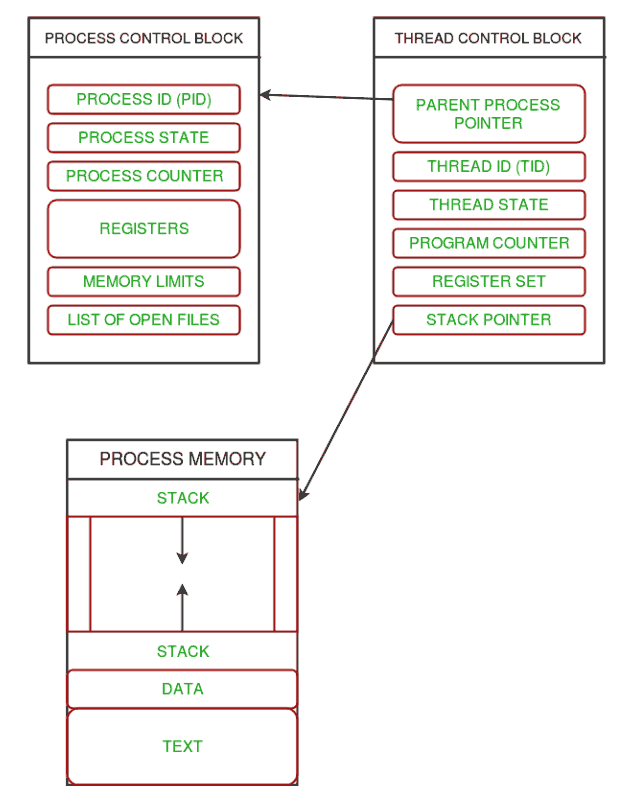
\includegraphics[scale=0.30]{multithreading_1.png}
	\end{minipage}
	\hspace{0.01\textwidth}
	\begin{minipage}{0.48\textwidth}
		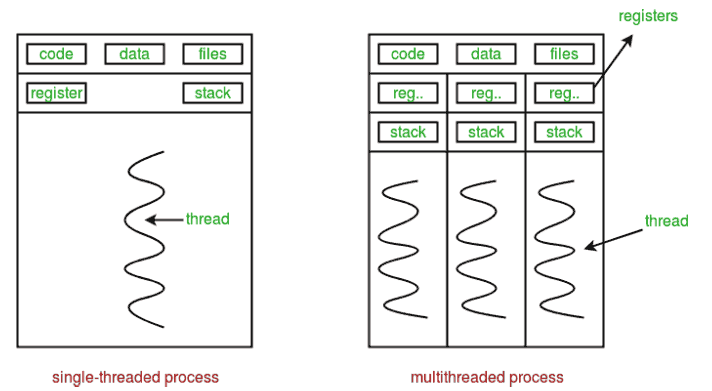
\includegraphics[scale=0.30]{multithreading_2.png}
	\end{minipage}
	\caption{Funzionamento di un thread: esso contiene tutte le informazioni dentro il TCB(\textbf{Thread Control Block}\index{TCB}) è identificato da un id che è unico, uno \emph{stack pointer} che punta invece alle variabili che sono definite dentro il namespace del thread, un parametro che identifica lo stato del thread e il \emph{parent process pointer} che invece punta al}
\end{figure}

\begin{wrapfigure}{l}{0.5\textwidth}
	\begin{lstlisting}[language=Python]
	import multiprocessing as mp
	
	def hello(q):
		q.put("Hello")
	if __name__ == "__main__":
		ctx = mp.getcontext("spawn")
		q = ctx.Queque()
		p = ctx.Process(target=foo, args=(q,))
    p.start()
    print(q.get())
    p.join()
	\end{lstlisting}
\caption{Esempio basilare di \emph{spawn} di un processo: un "processo" è semplicemente un'istanza della classe Oggetto, da cui è possibile andare a definire che argomenti passargli o altro}
\end{wrapfigure}

\noindent Come si può intuire da questo listato qua accanto, i processi sono creati utilizzando un oggetto \texttt{Process} e chiamando il metodo \texttt{.start} da cui possiamo, per esempio, andare a passare alcuni argomenti necessari alla funzione. \\
 
\end{document}